% =====================================================================
%  Capítulo 19. Datos de panel en finanzas
% =====================================================================
\chapter[Datos de panel]{Datos de panel en finanzas: efectos fijos, errores agrupados y paneles dinámicos}\label{cap:panel}

\section*{Objetivos de aprendizaje}
Al terminar este capítulo, el lector podrá:
\begin{enumerate}[label=\arabic*.,leftmargin=*]
  \item Estimar modelos de panel con MCO agrupado, efectos fijos, efectos aleatorios y primeras diferencias, y elegir
        entre ellos con la prueba de Hausman.
  \item Calcular errores estándar robustos a la correlación dentro de empresas, dentro de períodos o en ambas
        dimensiones, y saber cuál usar según la estructura de los datos (Petersen, 2009).
  \item Reconocer el sesgo de Nickell en los paneles dinámicos y corregirlo con variables instrumentales.
  \item Interpretar los efectos fijos de tiempo como una forma de aislar la variación de corte transversal, y relacionarlos
        con las regresiones de Fama y MacBeth.
\end{enumerate}

\section*{Motivación}
Buena parte de la investigación en finanzas corporativas y en valoración de activos usa paneles: muchas empresas
observadas durante muchos años, o muchas carteras observadas durante muchos meses. ¿Invierten más las empresas con
mayor valor de mercado? ¿Pagan los activos con mejor rendimiento pasado más rendimiento futuro? Un panel permite
controlar características de cada empresa que no se observan y que no cambian en el tiempo, y también choques comunes
a todas las empresas en un período. Pero los paneles financieros tienen una trampa: los residuos están correlacionados
dentro de cada empresa a lo largo del tiempo y dentro de cada período entre empresas. Petersen (2009) revisó los
artículos publicados en las tres principales revistas de finanzas y encontró que muchos ignoraban una u otra
correlación, con errores estándar subestimados.

\paragraph{Datos del capítulo.} Los datos de inversión de Grunfeld (1958): 10 grandes empresas industriales de EE.\,UU.
observadas de 1935 a 1954, con su inversión bruta, su valor de mercado y su stock de capital, en la versión de Baltagi
(2001). Y un panel de 30 carteras de Kenneth French (12 industrias, 9 de tamaño y valor y 9 de tamaño y momentum) con
807 meses, de enero de 1950 a marzo de 2017.

% ---------------------------------------------------------------------
\section{El modelo de efectos individuales}
% ---------------------------------------------------------------------

Sea $y_{it}$ la variable de la unidad $i=1,\dots,N$ en el período $t=1,\dots,T$. El modelo básico es
\[
  y_{it}=\mathbf x_{it}'\boldsymbol\beta+\alpha_i+\varepsilon_{it},
\]
donde $\alpha_i$ recoge todo lo que distingue a la unidad $i$ y no cambia en el tiempo: la calidad de la gerencia, la
tecnología del sector, la cultura de la empresa. Suponemos \emph{exogeneidad estricta}: $\E[\varepsilon_{it}\mid\mathbf
x_{i1},\dots,\mathbf x_{iT},\alpha_i]=0$. Lo que distingue a los estimadores es qué suponen sobre $\alpha_i$.

\paragraph{MCO agrupado.} Ignora $\alpha_i$ y estima por MCO con todas las observaciones. Es consistente solo si
$\alpha_i$ no está correlacionado con $\mathbf x_{it}$. Si las empresas con más valor de mercado tienen también, por
razones no observadas, más inversión, el estimador atribuye a $\mathbf x$ lo que es de $\alpha$ (Figura~\ref{fig:panelteoria}).

\paragraph{Efectos fijos (within).} Trata los $\alpha_i$ como parámetros y los elimina restando a cada variable su
media de la unidad, $\bar y_i=\frac1T\sum_ty_{it}$.

\begin{proposicion}[Estimador within]\label{prop:within}
Con $\ddot y_{it}=y_{it}-\bar y_i$ y $\ddot{\mathbf x}_{it}=\mathbf x_{it}-\bar{\mathbf x}_i$, el estimador
$\hat{\boldsymbol\beta}_W=(\sum_{i,t}\ddot{\mathbf x}_{it}\ddot{\mathbf x}_{it}')^{-1}\sum_{i,t}\ddot{\mathbf x}_{it}\ddot y_{it}$ es
insesgado bajo exogeneidad estricta, cualquiera sea la correlación entre $\alpha_i$ y $\mathbf x_{it}$.
\end{proposicion}

\begin{proof}
Promediando el modelo en el tiempo, $\bar y_i=\bar{\mathbf x}_i'\boldsymbol\beta+\alpha_i+\bar\varepsilon_i$. Restando:
\begin{align*}
  y_{it}-\bar y_i &= (\mathbf x_{it}-\bar{\mathbf x}_i)'\boldsymbol\beta+(\alpha_i-\alpha_i)+(\varepsilon_{it}-\bar\varepsilon_i)\\
  \ddot y_{it} &= \ddot{\mathbf x}_{it}'\boldsymbol\beta+\ddot\varepsilon_{it} .
\end{align*}
El efecto individual desaparece. Sustituyendo en el estimador:
\begin{align*}
  \hat{\boldsymbol\beta}_W &= \Bigl(\sum\ddot{\mathbf x}_{it}\ddot{\mathbf x}_{it}'\Bigr)^{-1}\sum\ddot{\mathbf x}_{it}(\ddot{\mathbf x}_{it}'\boldsymbol\beta+\ddot\varepsilon_{it})\\
                           &= \boldsymbol\beta+\Bigl(\sum\ddot{\mathbf x}_{it}\ddot{\mathbf x}_{it}'\Bigr)^{-1}\sum\ddot{\mathbf x}_{it}\ddot\varepsilon_{it}.
\end{align*}
Como $\ddot{\mathbf x}_{it}$ depende de $\mathbf x_{i1},\dots,\mathbf x_{iT}$ y $\ddot\varepsilon_{it}$ tiene esperanza condicional
cero dados esos valores (exogeneidad estricta), el segundo término tiene esperanza cero.
\end{proof}

El precio es que todo lo que no cambia en el tiempo desaparece junto con $\alpha_i$: no se puede estimar el efecto de una
característica fija de la empresa, y solo se usa la variación \emph{dentro} de cada unidad. Los grados de libertad para
$\hat\sigma^2_\varepsilon$ son $NT-N-K$, porque se estimaron implícitamente $N$ medias.

\paragraph{Primeras diferencias.} Otra forma de eliminar $\alpha_i$ es restar el período anterior:
$\Delta y_{it}=\Delta\mathbf x_{it}'\boldsymbol\beta+\Delta\varepsilon_{it}$. Con $T=2$, primeras diferencias y efectos fijos dan
exactamente el mismo estimador (Ejercicio propuesto 19.4); con $T>2$ difieren, y es más eficiente el within si los
$\varepsilon_{it}$ no están autocorrelacionados, y las diferencias si siguen un paseo aleatorio.

\paragraph{Efectos aleatorios.} Si se supone que $\alpha_i$ no está correlacionado con $\mathbf x_{it}$, con varianza
$\sigma_u^2$, el término compuesto $v_{it}=\alpha_i+\varepsilon_{it}$ tiene correlación $\sigma_u^2/(\sigma_u^2+\sigma_\varepsilon^2)$
entre dos períodos de la misma unidad, y el estimador eficiente es MCG.

\begin{proposicion}[Efectos aleatorios como cuasi-diferencia]\label{prop:re}
El estimador de MCG del modelo de efectos aleatorios es MCO sobre
$y_{it}-\theta\bar y_i=(1-\theta)\mu+(\mathbf x_{it}-\theta\bar{\mathbf x}_i)'\boldsymbol\beta+\text{error}$, con
\[
  \theta=1-\frac{\sigma_\varepsilon}{\sqrt{\sigma_\varepsilon^2+T\sigma_u^2}}.
\]
\end{proposicion}

\begin{proof}
Para la unidad $i$, la covarianza de $\mathbf v_i=(v_{i1},\dots,v_{iT})'$ es $\Omega=\sigma_\varepsilon^2I_T+\sigma_u^2\mathbf 1\mathbf 1'$. Con
$\bar J=\mathbf 1\mathbf 1'/T$ (la matriz que promedia) y $E=I-\bar J$ (la que resta la media), que son idempotentes,
ortogonales y suman $I$:
\begin{align*}
  \Omega &= \sigma_\varepsilon^2(E+\bar J)+T\sigma_u^2\bar J\\
         &= \sigma_\varepsilon^2E+(\sigma_\varepsilon^2+T\sigma_u^2)\bar J .
\end{align*}
Como $E$ y $\bar J$ son proyecciones ortogonales, cualquier potencia de $\Omega$ actúa sobre cada una por separado:
\begin{align*}
  \sigma_\varepsilon\,\Omega^{-1/2} &= E+\frac{\sigma_\varepsilon}{\sqrt{\sigma_\varepsilon^2+T\sigma_u^2}}\,\bar J\\
                                  &= I-\bar J+(1-\theta)\bar J\\
                                  &= I-\theta\bar J .
\end{align*}
Premultiplicar por $I-\theta\bar J$ resta $\theta$ veces la media de la unidad; MCO sobre los datos transformados es MCG.
\end{proof}

Si $\theta=0$ ($\sigma_u=0$), efectos aleatorios es MCO agrupado; si $\theta\to1$ ($T\sigma_u^2$ grande), se acerca a
efectos fijos. En la práctica, $\sigma_\varepsilon^2$ se estima con los residuos within y $\sigma_\varepsilon^2+T\sigma_u^2$ con los de
la regresión \emph{between} (de las medias $\bar y_i$ sobre $\bar{\mathbf x}_i$), el método de Swamy y Arora (1972).

\begin{proposicion}[Prueba de Hausman]\label{prop:hausman}
Bajo $H_0$: $\Cov(\alpha_i,\mathbf x_{it})=\mathbf 0$, ambos estimadores son consistentes y efectos aleatorios es eficiente. Entonces
$\Var(\hat{\boldsymbol\beta}_{FE}-\hat{\boldsymbol\beta}_{RE})=\Var(\hat{\boldsymbol\beta}_{FE})-\Var(\hat{\boldsymbol\beta}_{RE})$ y
\[
  H=(\hat{\boldsymbol\beta}_{FE}-\hat{\boldsymbol\beta}_{RE})'\bigl[\hat V_{FE}-\hat V_{RE}\bigr]^{-1}(\hat{\boldsymbol\beta}_{FE}-\hat{\boldsymbol\beta}_{RE})\ \xrightarrow{d}\ \chi^2_K .
\]
\end{proposicion}

\begin{proof}
Sea $\mathbf q=\hat{\boldsymbol\beta}_{FE}-\hat{\boldsymbol\beta}_{RE}$. El lema de Hausman dice que un estimador eficiente no está
correlacionado con su diferencia respecto de otro estimador consistente: $\Cov(\hat{\boldsymbol\beta}_{RE},\mathbf q)=\mathbf 0$ (si lo
estuviera, la combinación $\hat{\boldsymbol\beta}_{RE}+A\mathbf q$ con $A$ adecuada tendría menor varianza, contra la eficiencia).
Escribiendo $\hat{\boldsymbol\beta}_{FE}=\hat{\boldsymbol\beta}_{RE}+\mathbf q$:
\begin{align*}
  \Var(\hat{\boldsymbol\beta}_{FE}) &= \Var(\hat{\boldsymbol\beta}_{RE})+\Var(\mathbf q)+2\Cov(\hat{\boldsymbol\beta}_{RE},\mathbf q)\\
                                    &= \Var(\hat{\boldsymbol\beta}_{RE})+\Var(\mathbf q),\\
  \Var(\mathbf q) &= \Var(\hat{\boldsymbol\beta}_{FE})-\Var(\hat{\boldsymbol\beta}_{RE}).
\end{align*}
Como $\mathbf q$ es asintóticamente normal con media cero bajo $H_0$, la forma cuadrática con la inversa de su varianza es
$\chi^2_K$.
\end{proof}

Un rechazo indica que $\alpha_i$ está correlacionado con los regresores y que solo efectos fijos es consistente.

\paragraph{Agrupado, within y between.} El estimador agrupado mezcla las dos fuentes de variación.

\begin{proposicion}[Descomposición del estimador agrupado]\label{prop:mezclapanel}
Con un regresor, sean $S_W=\sum_{i,t}(x_{it}-\bar x_i)^2$ y $S_B=T\sum_i(\bar x_i-\bar x)^2$. Entonces
\[
  \hat\beta_{\text{agrupado}}=\frac{S_W}{S_W+S_B}\,\hat\beta_W+\frac{S_B}{S_W+S_B}\,\hat\beta_B .
\]
\end{proposicion}

\begin{proof}
La suma de cuadrados total se descompone en dentro y entre: $x_{it}-\bar x=(x_{it}-\bar x_i)+(\bar x_i-\bar x)$, y los
productos cruzados suman cero porque $\sum_t(x_{it}-\bar x_i)=0$. Lo mismo vale para los productos cruzados con $y$:
\begin{align*}
  \sum_{i,t}(x_{it}-\bar x)(y_{it}-\bar y) &= \sum_{i,t}(x_{it}-\bar x_i)(y_{it}-\bar y_i)+T\sum_i(\bar x_i-\bar x)(\bar y_i-\bar y)\\
                                           &= S_W\hat\beta_W+S_B\hat\beta_B,\\
  \sum_{i,t}(x_{it}-\bar x)^2 &= S_W+S_B .
\end{align*}
El estimador agrupado es el cociente de ambas expresiones.
\end{proof}

El mismo argumento vale si los grupos son períodos en lugar de unidades: con efectos fijos de \emph{tiempo}, solo se usa la
variación de corte transversal dentro de cada período. El Ejercicio~\ref{ej:descomposicion} muestra que esa distinción
cambia por completo la conclusión.

\begin{figure}[ht]
\centering
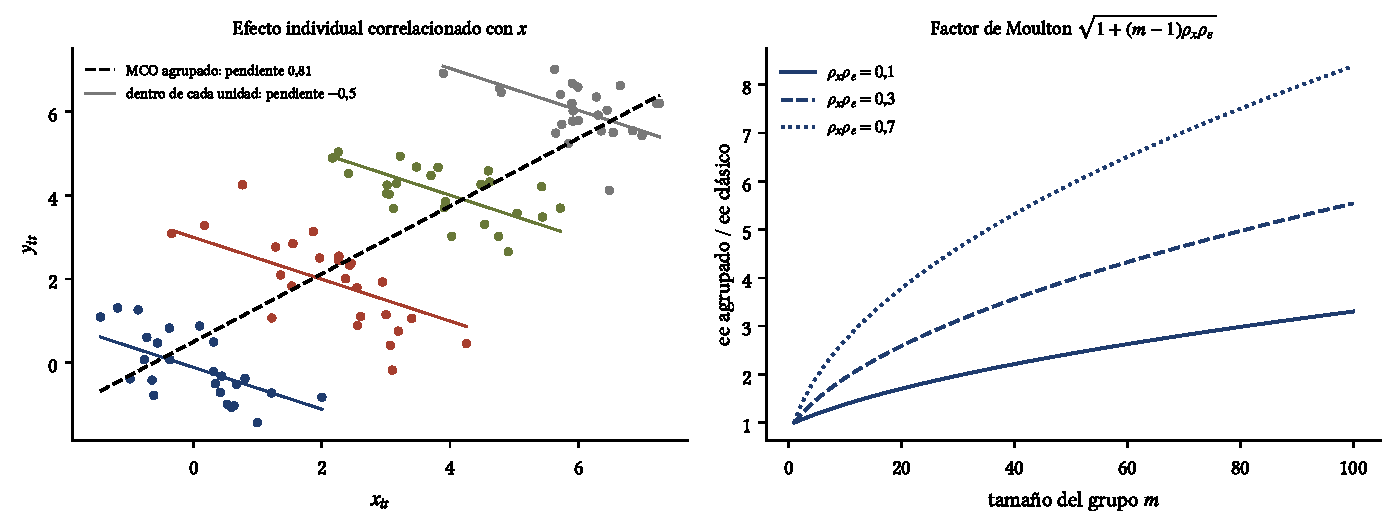
\includegraphics[width=\linewidth]{graficos/cap19_fig_teoria.pdf}
\caption{Izquierda: cuatro unidades con la misma pendiente, $-0{,}5$, pero con efectos individuales que crecen con $x$. El MCO
agrupado estima una pendiente positiva (0,81). Derecha: cuánto subestima el error estándar clásico cuando los residuos y el
regresor están correlacionados dentro de grupos de tamaño $m$.}
\label{fig:panelteoria}
\end{figure}

% ---------------------------------------------------------------------
\section{Errores estándar en paneles}
% ---------------------------------------------------------------------

Con cualquier estimador lineal $\hat{\boldsymbol\beta}=\boldsymbol\beta+(X'X)^{-1}X'\boldsymbol\varepsilon$, la varianza es
$(X'X)^{-1}X'\Omega X(X'X)^{-1}$. Lo que cambia es qué se supone sobre $\Omega=\Var(\boldsymbol\varepsilon\mid X)$:
\begin{itemize}[leftmargin=*]
  \item \textbf{Clásicos}: $\Omega=\sigma^2I$.
  \item \textbf{White}: $\Omega$ diagonal, con varianzas distintas.
  \item \textbf{Agrupados por $g$} (Liang y Zeger, 1986; Arellano, 1987): errores correlacionados de forma arbitraria dentro de
        cada grupo e independientes entre grupos, $\hat V=(X'X)^{-1}\bigl[\sum_gX_g'\hat{\boldsymbol\varepsilon}_g\hat{\boldsymbol\varepsilon}_g'X_g\bigr](X'X)^{-1}$,
        con el factor $\frac{G}{G-1}\frac{n-1}{n-K}$ en muestras finitas. Son consistentes cuando el número de grupos $G$ crece.
  \item \textbf{Dos vías} (Cameron, Gelbach y Miller, 2011; Thompson, 2011): $\hat V_{\text{empresa}}+\hat V_{\text{tiempo}}-\hat V_{\text{White}}$,
        para correlación dentro de empresas y dentro de períodos a la vez.
  \item \textbf{Driscoll y Kraay} (1998): Newey-West sobre la serie de tiempo $\mathbf h_t=\sum_i\mathbf x_{it}\hat\varepsilon_{it}$;
        robusto a correlación de corte transversal arbitraria y a autocorrelación hasta $L$ rezagos.
\end{itemize}

\begin{proposicion}[Factor de Moulton]\label{prop:moulton}
Sea un regresor $x$ y grupos de tamaño $m$ en los que, para dos observaciones distintas del mismo grupo,
\[
  \operatorname{Corr}(x_{it},x_{js})=\rho_x,\qquad \operatorname{Corr}(\varepsilon_{it},\varepsilon_{js})=\rho_\varepsilon
\]
(y cero entre grupos), con errores homocedásticos independientes de $x$. Entonces,
aproximadamente,
\[
  \frac{\Var_{\text{verdadera}}(\hat\beta)}{\Var_{\text{clásica}}(\hat\beta)}=1+(m-1)\rho_x\rho_\varepsilon .
\]
\end{proposicion}

\begin{proof}
Con $x$ centrado, $\hat\beta-\beta=\sum x_k\varepsilon_k/\sum x_k^2$. Condicionando en $x$, la varianza verdadera es
$\sum_k\sum_lx_kx_l\Cov(\varepsilon_k,\varepsilon_l)/(\sum x_k^2)^2$, y solo hay covarianzas dentro de los grupos:
\begin{align*}
  \sum_k\sum_lx_kx_l\Cov(\varepsilon_k,\varepsilon_l) &= \sigma^2\sum_kx_k^2+\rho_\varepsilon\sigma^2\sum_g\sum_{k\neq l\in g}x_kx_l .
\end{align*}
Con muchas observaciones, $\sum_g\sum_{k\neq l\in g}x_kx_l\approx(m-1)\rho_x\sum_kx_k^2$, porque cada observación tiene $m-1$
compañeras de grupo y el promedio de $x_kx_l$ entre compañeras es $\rho_x$ veces el de $x_k^2$:
\begin{align*}
  \Var_{\text{verdadera}}(\hat\beta) &\approx \frac{\sigma^2\sum_kx_k^2\,[1+(m-1)\rho_x\rho_\varepsilon]}{(\sum_kx_k^2)^2}\\
                                    &= \frac{\sigma^2}{\sum_kx_k^2}\,[1+(m-1)\rho_x\rho_\varepsilon]\\
                                    &= \Var_{\text{clásica}}(\hat\beta)\,[1+(m-1)\rho_x\rho_\varepsilon].
\end{align*}
\end{proof}

La consecuencia práctica (Moulton, 1990; Petersen, 2009) es que el sesgo de los errores clásicos solo es grande cuando
\emph{ambos}, el regresor y el residuo, están correlacionados dentro del grupo. En finanzas, el efecto empresa (una variable
persistente con un residuo persistente) pide agrupar por empresa; el efecto tiempo (un choque común que afecta a todas las
empresas en un mes y un regresor que también se mueve en común) pide agrupar por período. Con pocos grupos, por ejemplo 10
empresas, el estimador agrupado es poco fiable y conviene usar valores críticos de una $t$ con $G-1$ grados de libertad.

% ---------------------------------------------------------------------
\section{Paneles dinámicos}
% ---------------------------------------------------------------------

Si el modelo incluye la variable rezagada, $y_{it}=\rho y_{i,t-1}+\alpha_i+\varepsilon_{it}$, la exogeneidad estricta falla: $y_{i,t-1}$
depende de $\varepsilon_{i,t-1}$, que está en la media $\bar\varepsilon_i$ usada por el within. Nickell (1981) mostró que, con $N\to\infty$ y
$T$ fijo,
\[
  \operatorname{plim}\hat\rho_W-\rho\approx-\frac{1+\rho}{T-1},
\]
un sesgo negativo que solo desaparece cuando $T$ crece. Con $T=20$ y $\rho=0{,}7$, el sesgo es cercano a $-0{,}09$.

\begin{proposicion}[Instrumento de Anderson y Hsiao]\label{prop:ah}
En la ecuación en diferencias $\Delta y_{it}=\rho\,\Delta y_{i,t-1}+\Delta\varepsilon_{it}$, si los $\varepsilon_{it}$ no están
autocorrelacionados, $y_{i,t-2}$ es un instrumento válido para $\Delta y_{i,t-1}$.
\end{proposicion}

\begin{proof}
La diferencia elimina $\alpha_i$, pero $\Delta y_{i,t-1}=y_{i,t-1}-y_{i,t-2}$ está correlacionado con $\Delta\varepsilon_{it}=\varepsilon_{it}-\varepsilon_{i,t-1}$ a
través de $\varepsilon_{i,t-1}$. El nivel $y_{i,t-2}$ depende solo de $\alpha_i$ y de $\varepsilon_{i,t-2},\varepsilon_{i,t-3},\dots$:
\begin{align*}
  \E[y_{i,t-2}\,\Delta\varepsilon_{it}] &= \E[y_{i,t-2}\,\varepsilon_{it}]-\E[y_{i,t-2}\,\varepsilon_{i,t-1}]\\
                                         &= 0-0 .
\end{align*}
Y está correlacionado con $\Delta y_{i,t-1}$ (relevancia) mientras $\rho<1$, porque $\Delta y_{i,t-1}=(\rho-1)y_{i,t-2}+\alpha_i+\varepsilon_{i,t-1}$.
\end{proof}

Arellano y Bond (1991) usan como instrumentos todos los rezagos disponibles por el método generalizado de momentos, lo que
es más eficiente. Cuando $\rho$ es cercano a uno, los instrumentos en niveles son débiles y conviene el estimador de sistema de
Blundell y Bond (1998).

% ---------------------------------------------------------------------
\section{Ejercicios resueltos}
% ---------------------------------------------------------------------

\begin{ejresuelto}{La ecuación de inversión de Grunfeld}\label{ej:grunfeld}
\enunciado Estime $I_{it}=\beta_1F_{it}+\beta_2C_{it}+\alpha_i+\varepsilon_{it}$, donde $I$ es la inversión, $F$ el valor de mercado y $C$ el
stock de capital, con MCO agrupado, between, efectos fijos, efectos aleatorios y primeras diferencias. Contraste los efectos
individuales y aplique la prueba de Hausman.

\solucion
\paso{Paso 1. Estimaciones} (errores estándar clásicos entre paréntesis).
\begin{center}\small
\begin{tabular}{@{}lrr@{}}
\toprule
Estimador & Valor ($F$) & Capital ($C$) \\
\midrule
MCO agrupado & 0,1156 (0,0058) & 0,2307 (0,0255) \\
Between & 0,1346 (0,0287) & 0,0320 (0,1909) \\
Efectos fijos & 0,1101 (0,0119) & 0,3101 (0,0174) \\
Efectos aleatorios & 0,1098 (0,0105) & 0,3081 (0,0172) \\
Primeras diferencias & 0,0891 (0,0082) & 0,2787 (0,0472) \\
\bottomrule
\end{tabular}
\end{center}
Un millón más de valor de mercado se asocia con 0,11 millones más de inversión, y un millón más de capital, con 0,31. Las
estimaciones within coinciden con las de Baltagi (2001) y con \texttt{linearmodels}.

\paso{Paso 2. Efectos individuales.} La prueba $F$ de que los diez $\alpha_i$ son iguales:
\begin{align*}
  F &= \frac{(SCR_{\text{agrupado}}-SCR_W)/(N-1)}{SCR_W/(NT-N-K)}\\
    &= 49{,}18,
\end{align*}
con $(9,\,188)$ grados de libertad y valor $p$ de $10^{-44}$. Los efectos fijos estimados van de $-235{,}6$ a $101{,}9$.

\paso{Paso 3. Efectos aleatorios y Hausman.} Con $\hat\sigma_u=84{,}20$ y $\hat\sigma_\varepsilon=52{,}77$:
\begin{align*}
  \theta &= 1-\frac{52{,}77}{\sqrt{52{,}77^2+20\times84{,}20^2}}\\
         &= 1-\frac{52{,}77}{\sqrt{2\,784{,}7+141\,793}}\\
         &= 1-\frac{52{,}77}{380{,}23}\\
         &= 0{,}861 .
\end{align*}
Con $\theta$ tan cerca de uno, efectos aleatorios casi coincide con efectos fijos. El estadístico de Hausman es $H=2{,}33$ con valor
$p=0{,}31$: no se rechaza que los efectos sean aleatorios, y efectos aleatorios es preferible por eficiencia
(Figura~\ref{fig:grunfeld}).

\codigoweb{cap19_ej01}
\salidaR{cap19_ej01_R.txt}
\lectura{cap19_ej01}

\RvsPy La transformación within usa \texttt{ave(z, g)} en R, que devuelve la media del grupo repetida en cada observación, y una
función equivalente con \texttt{np.bincount} en Python. Los paquetes especializados son \texttt{plm} en R y \texttt{linearmodels}
en Python (\texttt{PanelOLS}, \texttt{RandomEffects}); con este último comprobamos los coeficientes de efectos fijos y aleatorios,
incluido $\theta=0{,}8612$. Las primeras diferencias requieren ordenar por empresa y año antes de restar.

\begin{figure}[ht]
\centering
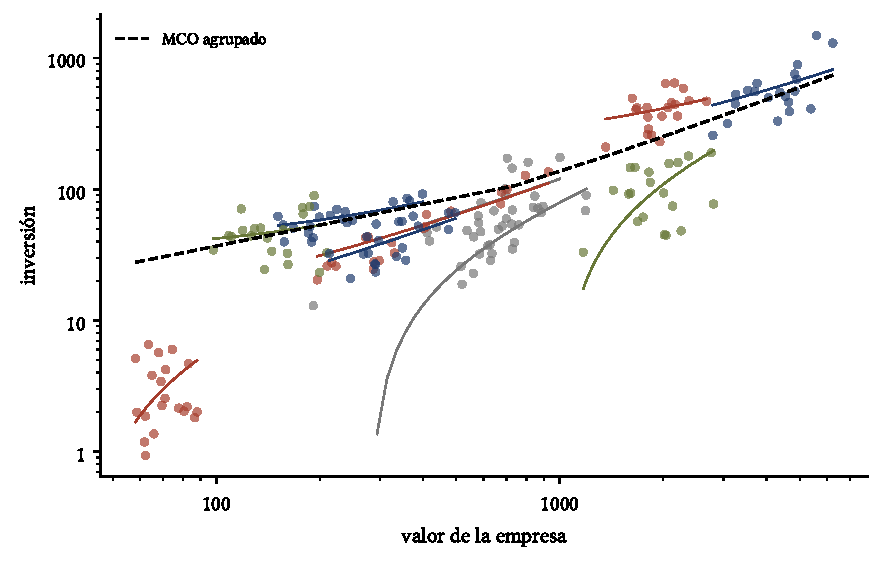
\includegraphics[width=0.78\linewidth]{graficos/cap19_ej01_grunfeld.pdf}
\caption{Inversión frente a valor de mercado de las 10 empresas (escala logarítmica), con las rectas de efectos fijos de cada empresa
(evaluadas en su capital medio y dibujadas donde la inversión ajustada es positiva) y la del MCO agrupado (discontinua).}
\label{fig:grunfeld}
\end{figure}

\begin{conclusion}
Las empresas difieren mucho en su nivel de inversión, pero esas diferencias no están correlacionadas con el valor y el capital lo
suficiente como para sesgar las pendientes: los cuatro estimadores consistentes con efectos individuales dan resultados similares,
y el MCO agrupado subestima el efecto del capital.
\end{conclusion}
\end{ejresuelto}

\begin{ejresuelto}{Errores estándar con pocas empresas}\label{ej:errores}
\enunciado Para el modelo de efectos fijos de Grunfeld, calcule los errores estándar clásicos, de White, agrupados por empresa, por
año, en dos vías y de Driscoll-Kraay. Estime también el modelo con efectos fijos de empresa y de año.

\solucion
\paso{Paso 1. La estructura de los residuos.} La autocorrelación media de orden 1 de los residuos de cada empresa es 0,632, y la
correlación media entre los residuos de dos empresas en el mismo año, 0,155: hay un efecto empresa fuerte y un efecto tiempo moderado.

\paso{Paso 2. Errores estándar.}
\begin{center}\small
\begin{tabular}{@{}lrrrr@{}}
\toprule
Método & ee(valor) & ee(capital) & $t$(valor) & $t$(capital) \\
\midrule
Clásicos & 0,0119 & 0,0174 & 9,29 & 17,87 \\
White & 0,0194 & 0,0428 & 5,68 & 7,25 \\
Agrupados por empresa & 0,0156 & 0,0540 & 7,08 & 5,74 \\
Agrupados por año & 0,0173 & 0,0323 & 6,36 & 9,61 \\
Dos vías & 0,0129 & 0,0461 & 8,53 & 6,72 \\
Driscoll-Kraay ($L=2$) & 0,0177 & 0,0348 & 6,23 & 8,90 \\
\bottomrule
\end{tabular}
\end{center}
El error estándar del capital se triplica al agrupar por empresa, coherente con la persistencia de los residuos. Aun así, todos los
coeficientes siguen siendo significativos, incluso con el valor crítico de la $t_9$ ($2{,}262$) que corresponde a 10 grupos.

\paso{Paso 3. Efectos de año.} Con efectos fijos de empresa y de año, $\hat\beta_F=0{,}1177$ y $\hat\beta_C=0{,}3579$. Los efectos de año van de
$+47{,}3$ (1935) a $-46{,}2$ (1954) respecto de la media, con un patrón descendente que recoge cambios comunes en la inversión que
no explican el valor y el capital.

\codigoweb{cap19_ej02}
\salidaR{cap19_ej02_R.txt}
\lectura{cap19_ej02}

\RvsPy Todas las matrices de varianza usan el mismo ``pan'' $(X'X)^{-1}$ y cambian el ``relleno''. En R, \texttt{sandwich::vcovCL}
y \texttt{sandwich::vcovPL} implementan los agrupados y Driscoll-Kraay; en Python, \texttt{linearmodels} con
\texttt{cov\_type="clustered"} o \texttt{"kernel"}. El factor de muestra finita varía entre programas (aquí, el de Stata), por lo
que conviene informar cuál se usa.

\begin{conclusion}
Los errores clásicos subestiman la incertidumbre hasta en un factor de tres. Con solo 10 empresas, ningún método agrupado es del
todo fiable: el panel de Grunfeld es largo y angosto, y los métodos de series de tiempo como Driscoll-Kraay son una alternativa
razonable.
\end{conclusion}
\end{ejresuelto}

\begin{ejresuelto}{El sesgo de Nickell}\label{ej:nickell}
\enunciado Estime $\ln I_{it}=\rho\ln I_{i,t-1}+\beta\ln F_{it}+\alpha_i+\varepsilon_{it}$ con MCO agrupado, efectos fijos y Anderson-Hsiao. Luego
simule 1\,000 paneles con $N=10$, $T=20$ y $\rho=0{,}7$ para medir el sesgo de efectos fijos.

\solucion
\paso{Paso 1. Datos reales.}
\begin{center}\small
\begin{tabular}{@{}lrrr@{}}
\toprule
Estimador & $\hat\rho$ & $\hat\beta$ & $n$ \\
\midrule
MCO agrupado & 0,914 (0,024) & 0,102 (0,028) & 190 \\
Efectos fijos & 0,700 (0,045) & 0,442 (0,076) & 190 \\
Anderson-Hsiao & 0,498 (0,288) & 0,691 (0,113) & 180 \\
\bottomrule
\end{tabular}
\end{center}
El MCO agrupado sobrestima la persistencia, porque atribuye a $\rho$ las diferencias permanentes entre empresas. Efectos fijos la
reduce, pero tiene sesgo de Nickell hacia abajo. Anderson-Hsiao es consistente, pero muy impreciso: su instrumento tiene una
correlación de apenas $-0{,}066$ con el regresor endógeno, un instrumento débil.

\paso{Paso 2. Simulación.} Con 19 observaciones efectivas por empresa, la fórmula de Nickell da
\begin{align*}
  -\frac{1+0{,}7}{19-1} &= -\frac{1{,}7}{18}\\
                       &= -0{,}094 .
\end{align*}
En la simulación, efectos fijos promedia $0{,}591$: un sesgo de $-0{,}109$, algo mayor que la aproximación (que es para $N$ grande), y
1,7 veces su desviación estándar (0,062). Anderson-Hsiao tiene una mediana de $0{,}711$, casi sin sesgo, pero con un rango
intercuartílico de 0,243, casi cuatro veces la desviación estándar de efectos fijos (Figura~\ref{fig:nickell}).

\codigoweb{cap19_ej03}
\salidaR{cap19_ej03_R.txt}
\lectura{cap19_ej03}

\RvsPy Los rezagos dentro de cada empresa se construyen con una tabla de búsqueda por (empresa, año): \texttt{match} con claves de
texto en R y un diccionario en Python, lo que evita mezclar el último año de una empresa con el primero de la siguiente. La
simulación usa el generador de Park y Miller con el método de Box y Muller, como en los Capítulos~\ref{cap:eventos}
y~\ref{cap:copulas}, y descarta 50 períodos iniciales.

\begin{figure}[ht]
\centering
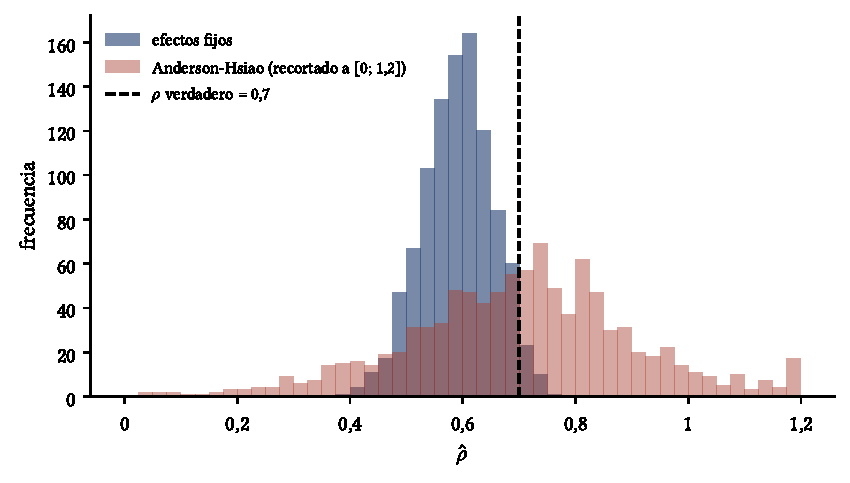
\includegraphics[width=0.78\linewidth]{graficos/cap19_ej03_nickell.pdf}
\caption{Distribución de $\hat\rho$ en 1\,000 paneles simulados con $N=10$, $T=20$ y $\rho=0{,}7$: efectos fijos (sesgado hacia abajo) y
Anderson-Hsiao (centrado, pero muy disperso).}
\label{fig:nickell}
\end{figure}

\begin{conclusion}
En paneles dinámicos cortos, efectos fijos subestima la persistencia y los estimadores de variables instrumentales la corrigen a
costa de mucha varianza. Con $T=20$ el sesgo de Nickell es comparable al error estándar, y no puede ignorarse.
\end{conclusion}
\end{ejresuelto}

\begin{ejresuelto}{¿Qué errores estándar? Un panel de carteras}\label{ej:petersen}
\enunciado Con el panel de 30 carteras y 807 meses, estime por MCO agrupado la regresión del exceso de rendimiento del mes $t$ sobre el
rendimiento acumulado de $t-12$ a $t-2$ (la señal de momentum). Compare los errores estándar de la pendiente con todos los métodos y
con Fama-MacBeth.

\solucion
\paso{Paso 1. Estructura de los datos.} Dentro de un mismo mes, los residuos de dos carteras tienen una correlación media de 0,708, y
la señal, de 0,700: un efecto tiempo enorme, porque todas las carteras se mueven con el mercado. En cambio, los residuos de una cartera
casi no están autocorrelacionados (0,101), aunque la señal sí lo está (0,921): el efecto cartera es pequeño.

\paso{Paso 2. Errores estándar.} La pendiente agrupada es $-0{,}00027$.
\begin{center}\small
\begin{tabular}{@{}lrrr@{}}
\toprule
Método & ee & $t$ & Cociente con el clásico \\
\midrule
Clásicos & 0,00180 & $-0{,}15$ & 1,00 \\
White & 0,00272 & $-0{,}10$ & 1,51 \\
Agrupados por cartera & 0,00117 & $-0{,}23$ & 0,65 \\
Agrupados por mes & 0,01038 & $-0{,}03$ & 5,75 \\
Dos vías & 0,01008 & $-0{,}03$ & 5,59 \\
Driscoll-Kraay ($L=12$) & 0,00921 & $-0{,}03$ & 5,10 \\
\midrule
Fama-MacBeth & 0,00430 & 6,18 & 2,38 \\
Fama-MacBeth con Newey-West & 0,00410 & 6,48 & 2,27 \\
\bottomrule
\end{tabular}
\end{center}
El error clásico subestima en un factor de casi 6 porque ignora el efecto tiempo. La Proposición~\ref{prop:moulton} lo anticipa:
\begin{align*}
  \sqrt{1+(30-1)\times0{,}700\times0{,}708} &= \sqrt{1+14{,}37}\\
                                             &= 3{,}92,
\end{align*}
que multiplicado por el factor de heterocedasticidad (1,51) da 5,9, cerca del 5,75 observado. Agrupar por cartera no sirve aquí:
el efecto cartera es débil y ese método ignora la correlación entre carteras.

\paso{Paso 3. Fama-MacBeth.} La pendiente media de las 807 regresiones de corte transversal es $0{,}02656$ con $t=6{,}18$: un resultado
opuesto al agrupado. No es un problema de errores estándar sino de \emph{qué se estima}, que es el tema del ejercicio siguiente. Las
pendientes mensuales casi no están autocorrelacionadas (0,099), por lo que la corrección de Newey-West apenas cambia el error
(Figura~\ref{fig:errores19}).

\codigoweb{cap19_ej04}
\salidaR{cap19_ej04_R.txt}
\lectura{cap19_ej04}

\RvsPy El panel se arma en formato largo, con una fila por cartera y mes, desde las matrices $T\times N$: \texttt{as.vector(t(R))} en R
recorre por filas como \texttt{R.ravel()} en Python. Las 807 pendientes de Fama-MacBeth salen de \texttt{lm} en R y de
\texttt{np.polyfit} en Python.

\begin{figure}[ht]
\centering
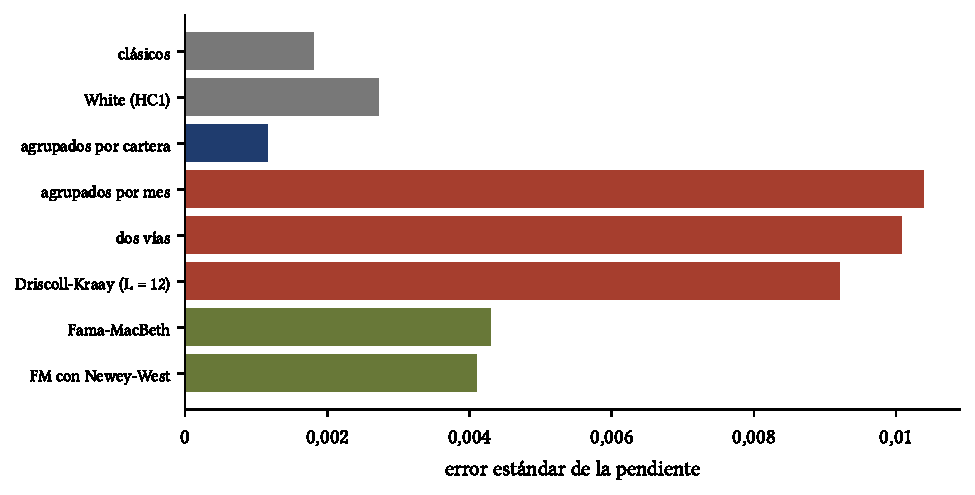
\includegraphics[width=0.85\linewidth]{graficos/cap19_ej04_errores.pdf}
\caption{Error estándar de la pendiente con cada método. Los que permiten correlación dentro del mes (rojo) son entre 5 y 6 veces el
clásico.}
\label{fig:errores19}
\end{figure}

\begin{conclusion}
En paneles de rendimientos, el efecto tiempo domina y los errores deben agruparse por período (o usar Driscoll-Kraay o
Fama-MacBeth). En paneles de finanzas corporativas, con variables persistentes como el apalancamiento, suele dominar el efecto empresa.
La regla de Petersen es calcular ambos y, si difieren, usar los de dos vías.
\end{conclusion}
\end{ejresuelto}

\begin{ejresuelto}{Momentum de series de tiempo y de corte transversal}\label{ej:descomposicion}
\enunciado Reestime la regresión del ejercicio anterior con efectos fijos de cartera, de mes y de ambos, con errores agrupados en dos
vías. Explique con la Proposición~\ref{prop:mezclapanel} por qué el estimador agrupado es casi cero.

\solucion
\paso{Paso 1. Especificaciones.}
\begin{center}\small
\begin{tabular}{@{}lrrrr@{}}
\toprule
Efectos fijos & Pendiente & ee (dos vías) & $t$ & Varianza de $x$ usada \\
\midrule
Ninguno & $-0{,}00027$ & 0,01008 & $-0{,}03$ & 1,000 \\
Cartera & $-0{,}00251$ & 0,01021 & $-0{,}25$ & 0,976 \\
Mes & 0,01634 & 0,00673 & 2,43 & 0,327 \\
Cartera y mes & 0,01045 & 0,00667 & 1,57 & 0,303 \\
\bottomrule
\end{tabular}
\end{center}
Con efectos de mes, solo se compara cada cartera con las demás \emph{en el mismo mes}: las de mejor rendimiento pasado rinden más
después, el momentum de corte transversal de Jegadeesh y Titman (1993). Diez puntos más de rendimiento pasado anticipan 0,163 puntos
más de rendimiento mensual.

\paso{Paso 2. La descomposición.} El 67,3\,\% de la varianza de la señal es \emph{entre meses} (todas las carteras subieron o bajaron
juntas), y en esa dimensión la relación es negativa: la regresión del rendimiento medio del mes sobre la señal media da $-0{,}00834$. Por
la Proposición~\ref{prop:mezclapanel}, con los meses como grupos:
\begin{align*}
  \hat\beta_{\text{agrupado}} &= 0{,}3270\times0{,}01634+0{,}6730\times(-0{,}00834)\\
                              &= 0{,}00534-0{,}00561\\
                              &= -0{,}00027 .
\end{align*}
Los dos efectos se cancelan. El MCO agrupado, que parecía decir que el momentum no existe, promedia una relación de corte transversal
positiva con una de series de tiempo del mercado negativa (Figura~\ref{fig:descomposicion}).

\paso{Paso 3. Relación con Fama-MacBeth.} Efectos fijos de mes y Fama-MacBeth usan la misma variación de corte transversal, pero
ponderan los meses de forma distinta: Fama-MacBeth da igual peso a cada mes, y la regresión con efectos de mes pondera cada mes por la
dispersión de la señal en ese mes. Por eso sus pendientes difieren (0,0266 y 0,0163) aunque ambas son positivas.

\codigoweb{cap19_ej05}
\salidaR{cap19_ej05_R.txt}
\lectura{cap19_ej05}

\RvsPy Con un panel balanceado, los efectos fijos en dos vías se eliminan restando las medias de cartera y de mes y sumando la media
total; con un panel desbalanceado esa fórmula no es exacta y hay que iterar o usar ficticias. Los grados de libertad que restan los
efectos fijos ($N-1$ y $T-1$) se descuentan en el factor de muestra finita de los errores agrupados.

\begin{figure}[ht]
\centering
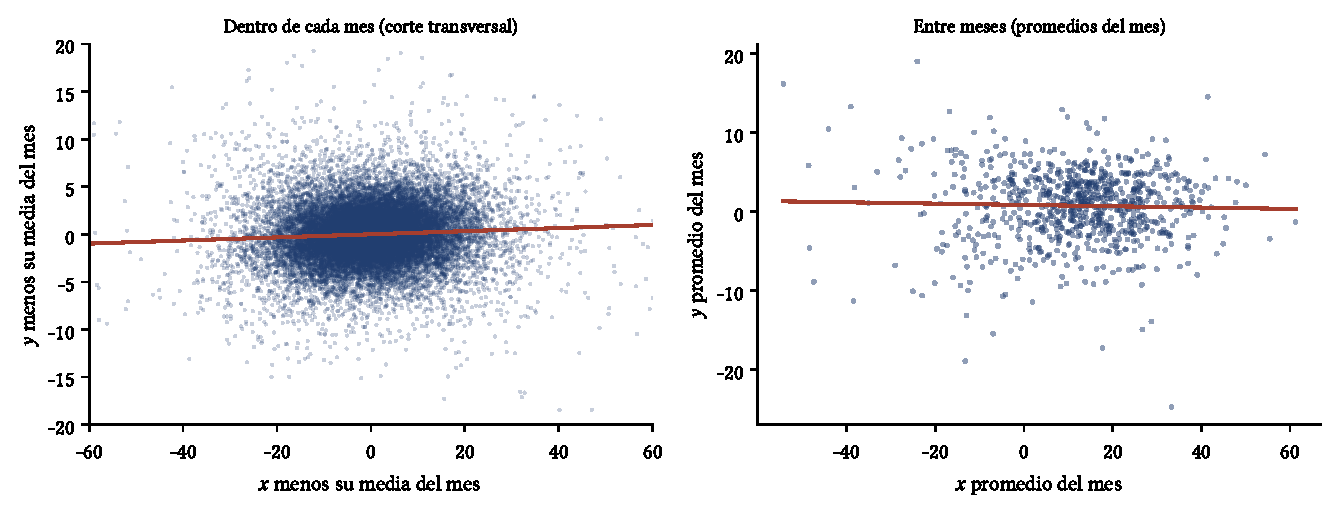
\includegraphics[width=\linewidth]{graficos/cap19_ej05_descomposicion.pdf}
\caption{Izquierda: relación de corte transversal (desviaciones respecto de la media del mes), con pendiente positiva. Derecha: relación
entre meses (promedios de las 30 carteras), con pendiente negativa.}
\label{fig:descomposicion}
\end{figure}

\begin{conclusion}
Los efectos fijos no son solo un control: deciden qué variación identifica el coeficiente. En valoración de activos, la pregunta suele
ser de corte transversal, y la especificación correcta incluye efectos de período o usa Fama-MacBeth.
\end{conclusion}
\end{ejresuelto}

% ---------------------------------------------------------------------
\section{Ejercicios propuestos}
% ---------------------------------------------------------------------

\begin{enumerate}[label=\textbf{\thechapter.\arabic*},leftmargin=*,itemsep=6pt]
  \item Con $\sigma_\varepsilon=2$, $\sigma_u=3$ y $T=8$, calcule $\theta$ del estimador de efectos aleatorios. \textit{Respuesta:
  $1-2/\sqrt{4+72}=0{,}7706$.}

  \item En un panel de 50 empresas y 20 años, la correlación de los residuos dentro de cada empresa es 0,4 y la del regresor, 0,8.
  ¿Cuánto subestiman los errores clásicos? \textit{Respuesta: un factor de $\sqrt{1+19\times0{,}32}=2{,}66$.}

  \item Con $T=10$ y $\rho=0{,}5$, calcule el sesgo aproximado de Nickell. \textit{Respuesta: $-1{,}5/9=-0{,}167$.}

  \item Demuestre que con $T=2$ el estimador de efectos fijos y el de primeras diferencias son idénticos.

  \item Demuestre la versión matricial de la Proposición~\ref{prop:mezclapanel}:
  $\hat{\boldsymbol\beta}_{\text{agrupado}}=(S_W+S_B)^{-1}(S_W\hat{\boldsymbol\beta}_W+S_B\hat{\boldsymbol\beta}_B)$, con $S_W$ y $S_B$ matrices.

  \item \emph{(Simulación.)} Simule paneles de 500 empresas y 10 años con efecto empresa ($\rho_x=\rho_\varepsilon=0{,}5$) y estime la frecuencia de
  rechazo al 5\,\% de una hipótesis verdadera con errores clásicos, de White y agrupados por empresa (Petersen, 2009).

  \item \emph{(Con datos de la SMV.)} Con los estados financieros de las empresas listadas en la BVL, estime la relación entre
  apalancamiento y rentabilidad con efectos fijos de empresa y de año. ¿Qué dimensión de agrupamiento importa más?

  \item \emph{(Con datos.)} Repita el Ejercicio~\ref{ej:descomposicion} usando solo las 12 industrias. ¿Hay momentum de industrias
  (Moskowitz y Grinblatt, 1999)?
\end{enumerate}

% ---------------------------------------------------------------------
\section{Resumen de fórmulas}
% ---------------------------------------------------------------------

\begin{table}[H]
\centering\small
\begin{tabular}{@{}ll@{}}
\toprule
Concepto & Fórmula \\
\midrule
Within & $\ddot y_{it}=y_{it}-\bar y_i$;\quad $\hat{\boldsymbol\beta}_W=(\sum\ddot{\mathbf x}\ddot{\mathbf x}')^{-1}\sum\ddot{\mathbf x}\ddot y$;\quad gl $=NT-N-K$ \\
Efectos aleatorios & $y_{it}-\theta\bar y_i$;\quad $\theta=1-\sigma_\varepsilon/\sqrt{\sigma_\varepsilon^2+T\sigma_u^2}$ \\
Hausman & $(\hat{\boldsymbol\beta}_{FE}-\hat{\boldsymbol\beta}_{RE})'[\hat V_{FE}-\hat V_{RE}]^{-1}(\cdot)\sim\chi^2_K$ \\
Agrupado = mezcla & $\hat\beta=\frac{S_W}{S_W+S_B}\hat\beta_W+\frac{S_B}{S_W+S_B}\hat\beta_B$ \\
Errores agrupados & $(X'X)^{-1}\sum_gX_g'\hat{\boldsymbol\varepsilon}_g\hat{\boldsymbol\varepsilon}_g'X_g(X'X)^{-1}\cdot\frac{G}{G-1}\frac{n-1}{n-K}$ \\
Dos vías & $\hat V_{\text{empresa}}+\hat V_{\text{tiempo}}-\hat V_{\text{White}}$ \\
Factor de Moulton & $1+(m-1)\rho_x\rho_\varepsilon$ \\
Sesgo de Nickell & $\approx-(1+\rho)/(T-1)$ \\
Anderson-Hsiao & $\Delta y_{it}=\rho\Delta y_{i,t-1}+\Delta\varepsilon_{it}$, instrumento $y_{i,t-2}$ \\
\bottomrule
\end{tabular}
\caption{Fórmulas principales del Capítulo 19.}
\end{table}

\section*{Referencias}
\begin{itemize}[leftmargin=*]
  \item Anderson, T. W. y Hsiao, C. (1981). Estimation of dynamic models with error components. \emph{Journal of the American
        Statistical Association}, 76(375), 598--606.
  \item Arellano, M. (1987). Computing robust standard errors for within-groups estimators. \emph{Oxford Bulletin of Economics and
        Statistics}, 49(4), 431--434.
  \item Arellano, M. y Bond, S. (1991). Some tests of specification for panel data: Monte Carlo evidence and an application to
        employment equations. \emph{Review of Economic Studies}, 58(2), 277--297.
  \item Baltagi, B. H. (2001). \emph{Econometric Analysis of Panel Data}, 3.ª ed. Wiley.
  \item Blundell, R. y Bond, S. (1998). Initial conditions and moment restrictions in dynamic panel data models. \emph{Journal of
        Econometrics}, 87(1), 115--143.
  \item Cameron, A. C., Gelbach, J. B. y Miller, D. L. (2011). Robust inference with multiway clustering. \emph{Journal of
        Business \& Economic Statistics}, 29(2), 238--249.
  \item Driscoll, J. C. y Kraay, A. C. (1998). Consistent covariance matrix estimation with spatially dependent panel data.
        \emph{Review of Economics and Statistics}, 80(4), 549--560.
  \item Grunfeld, Y. (1958). \emph{The Determinants of Corporate Investment}. Tesis doctoral, Universidad de Chicago.
  \item Hausman, J. A. (1978). Specification tests in econometrics. \emph{Econometrica}, 46(6), 1251--1271.
  \item Jegadeesh, N. y Titman, S. (1993). Returns to buying winners and selling losers: Implications for stock market
        efficiency. \emph{Journal of Finance}, 48(1), 65--91.
  \item Kleiber, C. y Zeileis, A. (2010). The Grunfeld data at 50. \emph{German Economic Review}, 11(4), 404--417.
  \item Liang, K.-Y. y Zeger, S. L. (1986). Longitudinal data analysis using generalized linear models. \emph{Biometrika}, 73(1),
        13--22.
  \item Moskowitz, T. J. y Grinblatt, M. (1999). Do industries explain momentum? \emph{Journal of Finance}, 54(4), 1249--1290.
  \item Moulton, B. R. (1990). An illustration of a pitfall in estimating the effects of aggregate variables on micro units.
        \emph{Review of Economics and Statistics}, 72(2), 334--338.
  \item Nickell, S. (1981). Biases in dynamic models with fixed effects. \emph{Econometrica}, 49(6), 1417--1426.
  \item Petersen, M. A. (2009). Estimating standard errors in finance panel data sets: Comparing approaches. \emph{Review of
        Financial Studies}, 22(1), 435--480.
  \item Swamy, P. A. V. B. y Arora, S. S. (1972). The exact finite sample properties of the estimators of coefficients in the error
        components regression models. \emph{Econometrica}, 40(2), 261--275.
  \item Thompson, S. B. (2011). Simple formulas for standard errors that cluster by both firm and time. \emph{Journal of Financial
        Economics}, 99(1), 1--10.
\end{itemize}
